\documentclass[12pt,a4paper,reqno]{report}
\usepackage{mystyle}


\begin{document}
\begin{titlepage}

\centering

\includegraphics[width=\textwidth]{images/FrontPage/ITU_logo_en.jpg}
	\textcolor{black}{\rule{\linewidth}{1pt}} \par
     {\scshape\Huge\bfseries \textcolor{black}{Final Report}\par} 
	\vspace{1pt}
	IT-University of Copenhagen
	\textcolor{black}{\rule{\linewidth}{1pt}} \par
	\vspace*{0.25cm}
 \textbf{Course Name:} DevOps: Software Evolution and Software Maintenance\\
\textbf{Course Code:} KSDSESM1KU\\
\textbf{Submission Date:} 30/05/2025\\
\textbf{Group i - CloudMorphers} \\
 
\vspace*{1cm}
 
\begin{minipage}{0.75\textwidth}
    \begin{flushleft}
        \textbf{Authors}\\
        Alexander Niclas Lerche\\
        Cem Ergin\\
        Lucian-Alexandru Aionicesei\\
        Philip Mørch
    \end{flushleft}
    \end{minipage}
    \begin{minipage}{0.20\textwidth}
    \begin{flushright}
        \textbf{Email}\\
        alnl@itu.dk\\
        ceme@itu.dk\\
        laio@itu.dk\\
        phimo@itu.dk
    \end{flushright}
\end{minipage}

\end{titlepage}
 
\clearpage
\tableofcontents
\addtocontents{toc}{\vspace{-0.5cm}}

\setcounter{page}{0}
\clearpage 

%\clearpage
\section*{Abstract}
At the start of the project, we chose to replace the original Flask-React application with a new implementation in ASP.NET Core. This was a complete rewrite, as it involved changing both the front-end and back-end technology stacks and reimplementing functionality from scratch.

\section{System Perspective}

\subsection{Design and Architecture}
% Design and architecture of your ITU-MiniTwit systems

% Overview description and diagram of the system
% - Web frontend
% - Backend API
% - Database

Initially, when we took over MiniTwit, it was a Python-based application built with the Flask framework. We then began to replace it with a new implementation using ASP.NET Core. As some group members already had experience using C\# and found that it had a nice ecosystem. All other members had experience with Java but wanted to learn C\#, we felt this was a beneficial decision for both the project and our learning as students. This was a complete rewrite, as it involved changing both the front-end and back-end technology stacks and reimplementing functionality from scratch.

\subsubsection{The Frontend}
For the front-end of our Minitwit application, we use ASP.NET Core MVC architecture. We choose this as this pattern supports a clean structure and allows us to build the app in a way that is both easily maintainable and testable. According to Anderson (2025), the MVC pattern improves maintainability by separating concerns, helping make applications more testable and easier to update than traditional monolithic apps.

\subsubsection{The Backend}
Our backend, which is built on ASP.NET Core and follows the MVC architecture, is responsible for handling requests, processing data, and connecting to the database. This allows us to separate responsibilities between our applications domain models (Models), routing and logic (Controllers), and data access (Data). We organized it so that we have multiple controllers with different responsibilities.

\subsubsection{The Database}

\subsection{Dependencies (across all levels)}
% All dependencies of your ITU-MiniTwit systems on all levels of abstraction and development stages. That is, list and briefly describe all technologies and tools you applied and depend on.

We generated a dependency graph with NDepend, a static analysis tool for .NET projects that helps visualize code dependencies and measure quality: \href{http://67.207.72.20:8081/NDependReportFiles/ComponentDependenciesDiagram.html}{dependency-diagram}.

\vspace*{0.5cm}

\begin{figure}[h!]
    \centering
    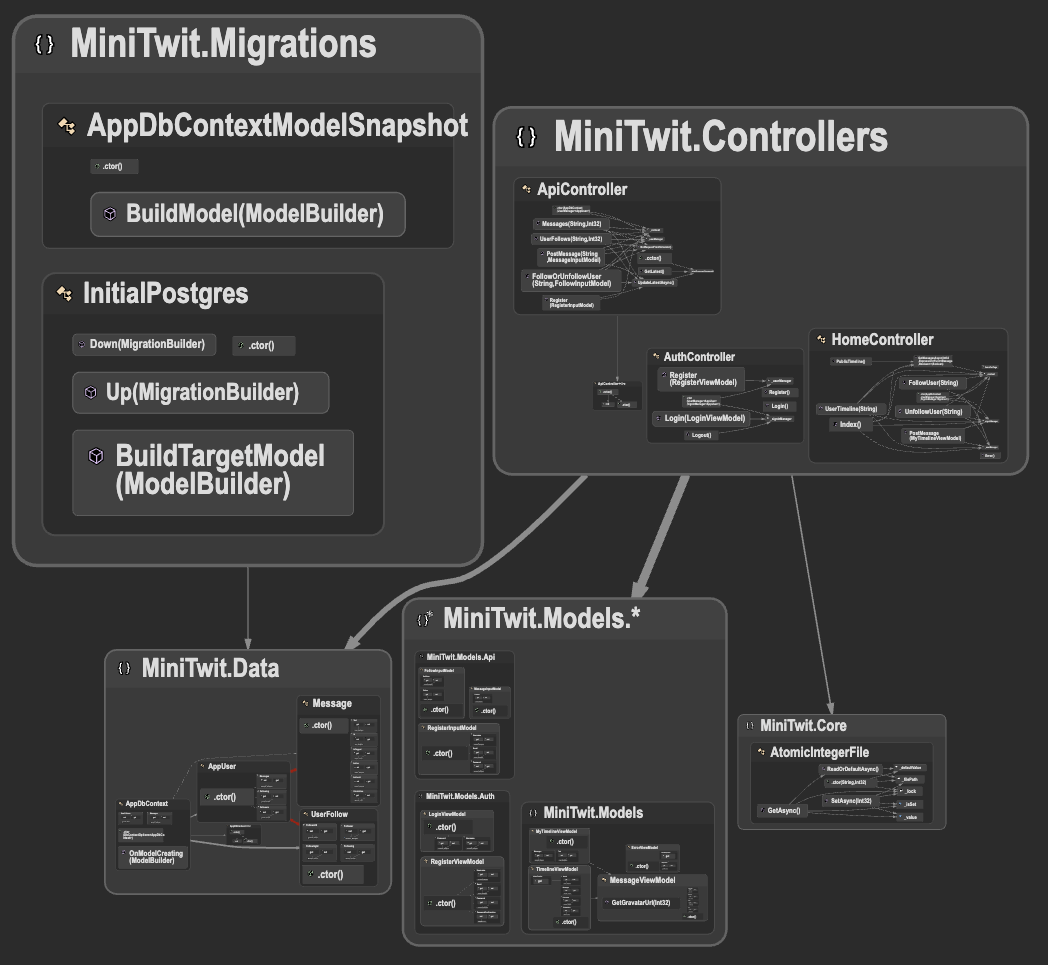
\includegraphics[width=0.75\textwidth]{images/MiniTwit-DependencyDiagram.png}
    \caption{Dependency diagram of the MiniTwit system.}
    \label{fig:minitwit-diagram}
\end{figure}

The diagram visualizes the internal structure of the codebase by showing how the namespaces depend on each other. The architecture is organized into distinct layers: Controllers, Models, Data, Migrations, and Core.

The project follows the Model-View-Controller (MVC) pattern. Controllers handle HTTP requests and interact with Models, which represent the application data structures. The Data layer is responsible for data access and persistence; although not explicitly shown in the diagram, it uses Entity Framework Core to communicate with the database.

\vspace*{0.5cm}

\begin{figure}[h!]
    \centering
    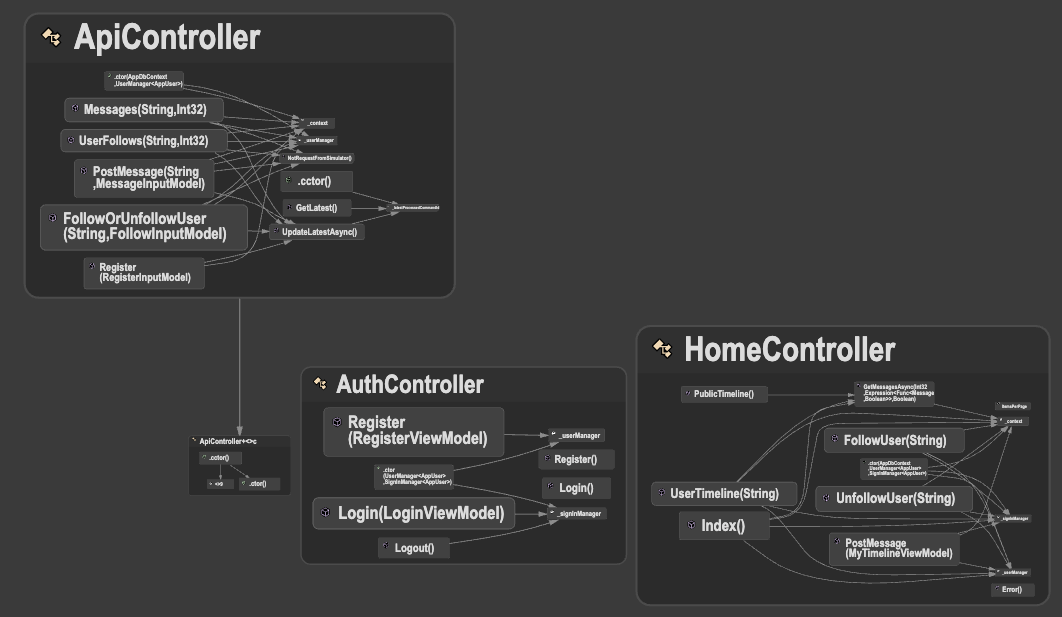
\includegraphics[width=0.85\textwidth]{images/MiniTwitControllers-DependencyDiagram.png}
    \caption{Dependency diagram of the MiniTwit controllers.}
    \label{fig:minitwit-diagram}
\end{figure}

The Controllers layer is further divided into specific controllers based on functionality: ApiController handles API requests, AuthController manages authentication and user access, and HomeController serves the main web pages. This separation helps organize concerns and simplifies maintenance by clearly delineating different parts of the application interface.

\subsection{Important Interactions of Subsystems}
% Important interactions of subsystems.

% - For example, via an illustrative UML Sequence diagram that shows the flow of information through your system from user request in the browser, over all subsystems, hitting the database, and a response that is returned to the user.
% - Similarly, another illustrative sequence diagram that shows how requests from the simulator traverse your system.

The system handles two key interaction flows, captured in the provided UML sequence diagrams.

\begin{figure}[h!]
    \centering
    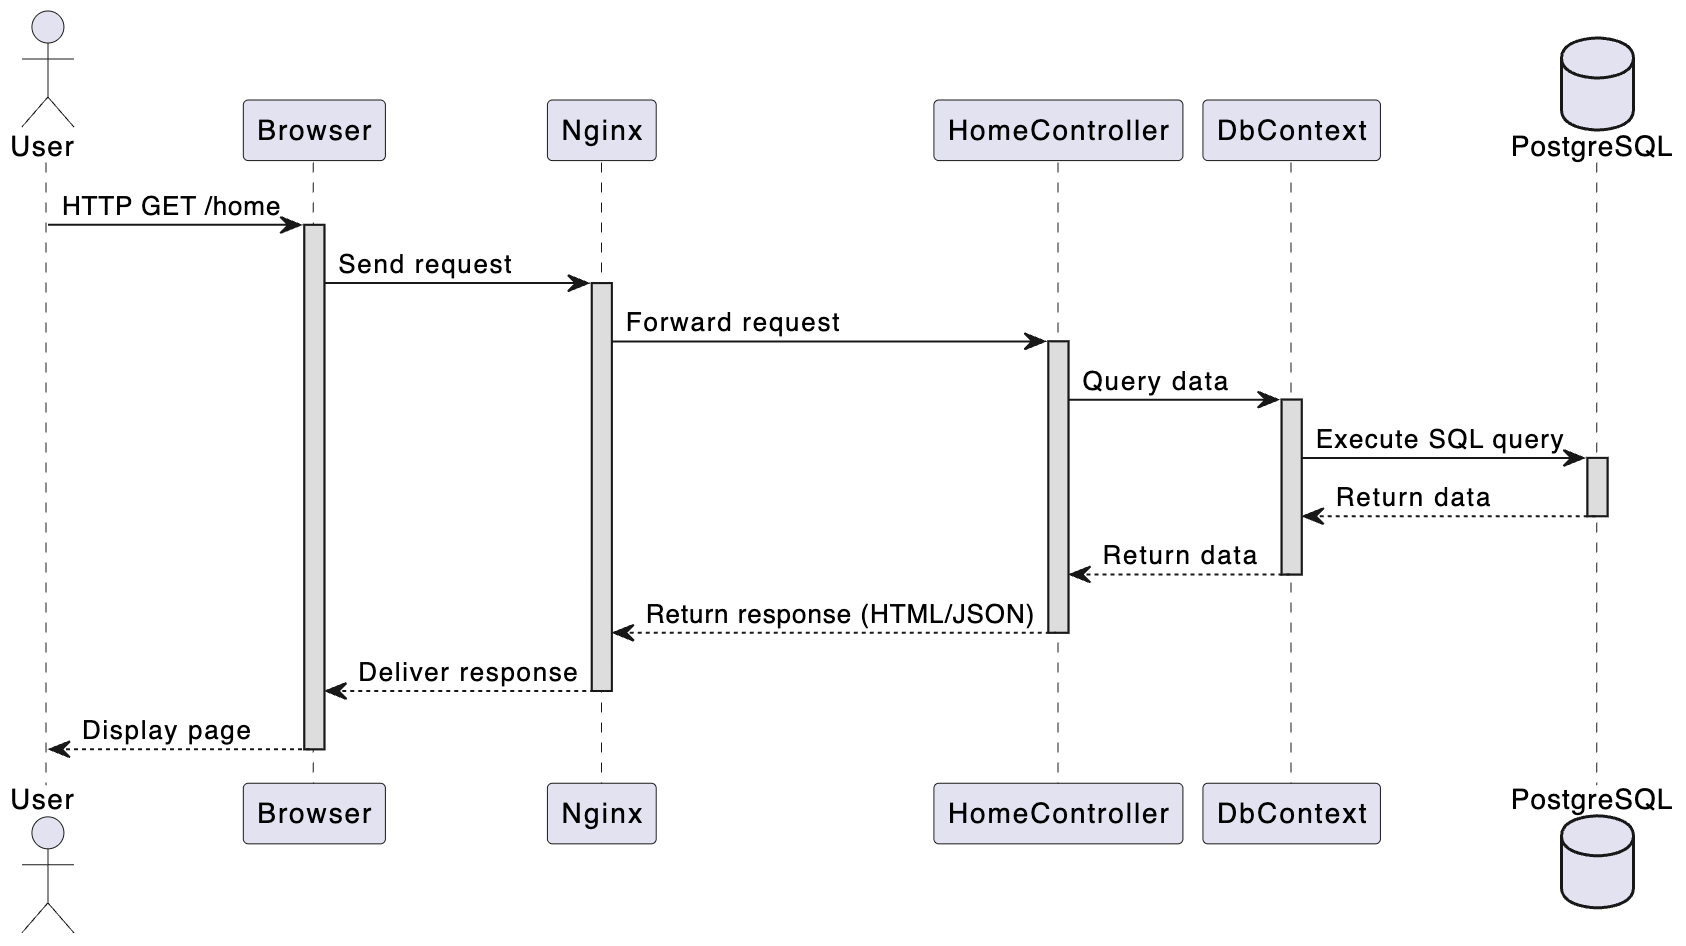
\includegraphics[width=\textwidth]{images/user-interaction-uml.png}
    \caption{User interaction sequence diagram.}
    \label{fig:minitwit-diagram}
\end{figure}

In the first flow, a user sends a request from the browser (e.g., accessing the home page or registering). This request is routed through Nginx, which forwards it to the HomeController or AuthController of the ASP.NET Core application. The controller uses the Entity Framework DbContext to query or update the PostgreSQL database. Once the database returns the result, the controller prepares the response, which is passed back through Nginx to the browser, ultimately presenting the result to the user.

\begin{figure}[h!]
    \centering
    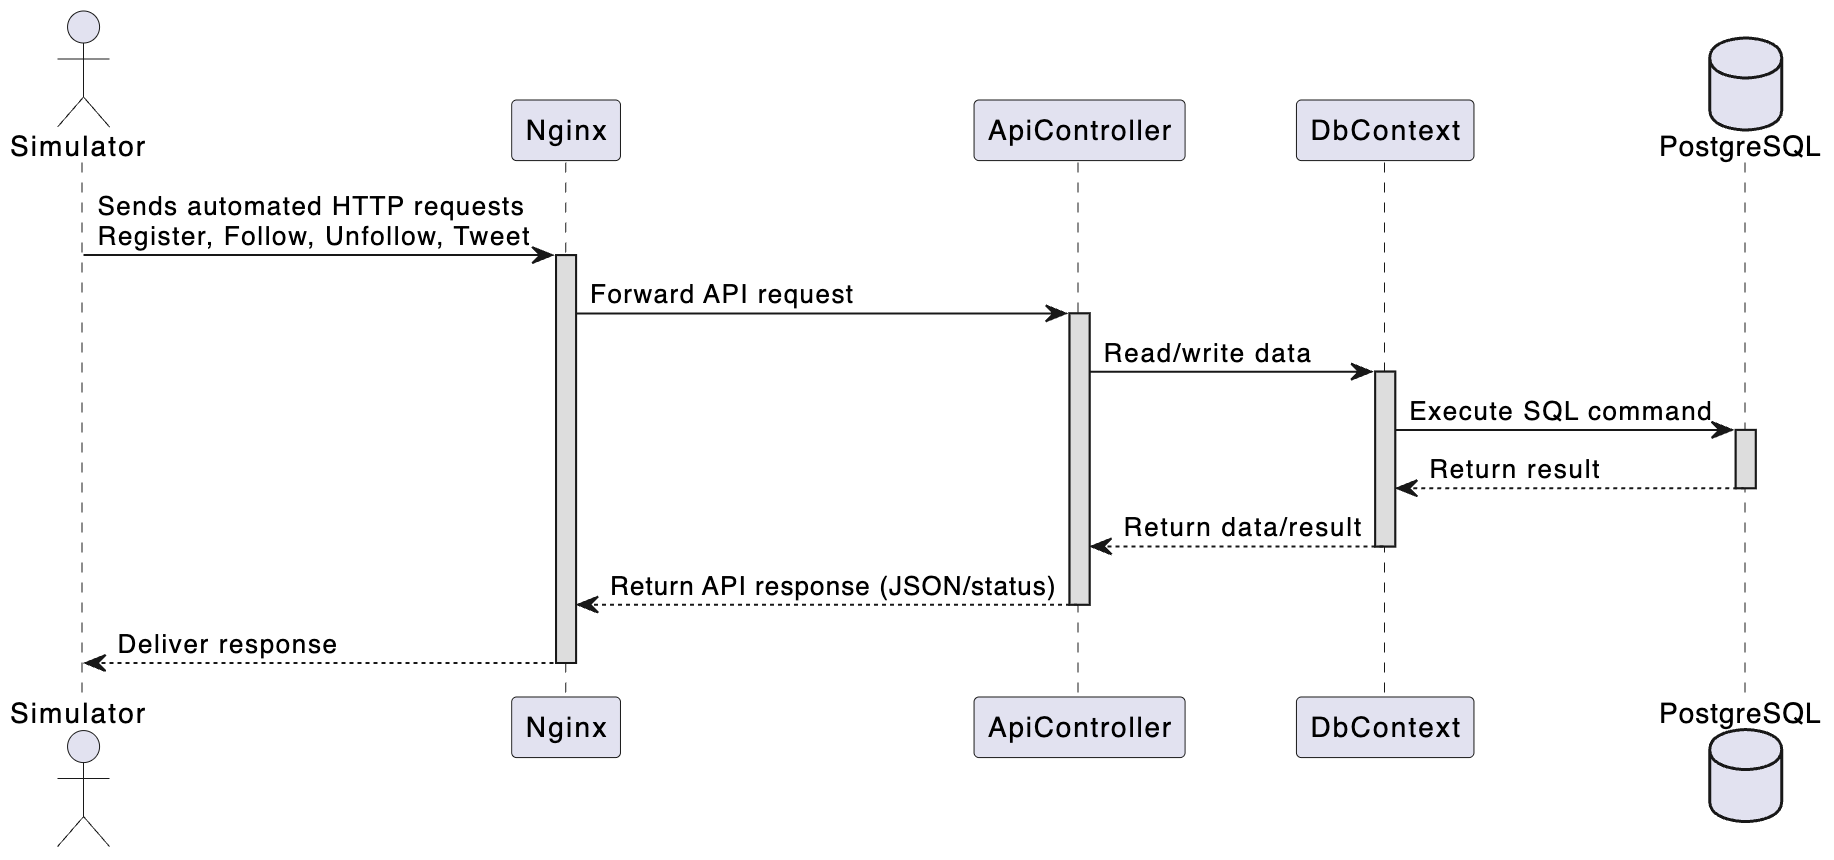
\includegraphics[width=\textwidth]{images/simulator-interaction-uml.png}
    \caption{Simulator interaction sequence diagram.}
    \label{fig:minitwit-diagram}
\end{figure}

In the second flow, the simulator (used to mimic user behavior) sends API requests to the system. These requests also pass through Nginx but are handled by the ApiController. Like the HomeController, it interacts with the DbContext and the PostgreSQL database. The system processes the simulator’s requests and returns JSON responses, ensuring the simulator can effectively test user interactions and system behavior under load.

The DbContext is the data access layer of the system, provided by the Entity Framework Core. It connects the application’s C\# models to the PostgreSQL database, translating high-level queries and operations into SQL commands. This allows controllers to manage data without handling raw SQL, ensuring maintainable code.

This flow shows the main subsystem interaction: the external simulator triggering API endpoints, the application back-end handling business logic, and the database layer executing the necessary data operations.

\subsection{Current State}
% Describe the current state of your systems, for example using results of static analysis and quality assessments.

Our ASP.Net Core application is built and deployed through a CI/CD pipeline using GitHub Actions and Docker, automating building, publishing, and containerization. However, static code quality checks are currently limited.

To assess the codebase’s quality, we ran a local static analysis using NDepend, which produced detailed dependency diagrams and metrics on system health. Although not integrated into the CI/CD workflow, the HTML report is hosted on the server for team review: \href{http://67.207.72.20:8081/NDependReport.html#Main}{NDependReport}.

\begin{figure}[h!]
    \centering
    % Left block: two stacked images
    \begin{minipage}[b]{0.42\textwidth}
        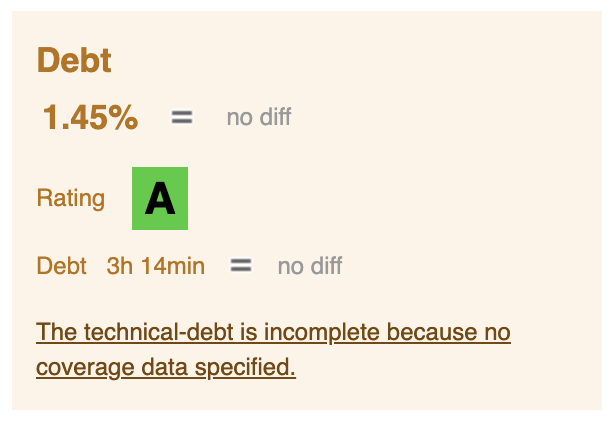
\includegraphics[width=\textwidth]{images/Technical-debt-estimation.png} \\[1ex]
        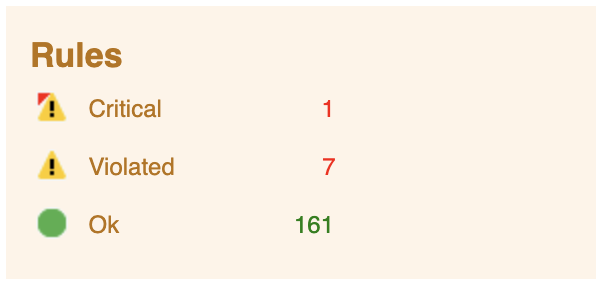
\includegraphics[width=\textwidth]{images/Rules.png}
    \end{minipage}
    \hspace{0.5ex}
    % Right block: one tall image
    \begin{minipage}[b]{0.53\textwidth}
        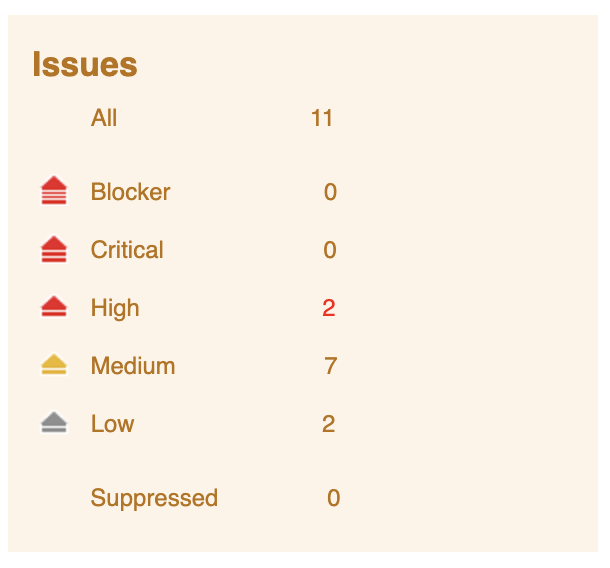
\includegraphics[width=\textwidth]{images/Issues.png}
    \end{minipage}
    \caption{Overview of NDepend Static Analysis Results }
    \label{fig:composite}
\end{figure}

The analysis indicates low technical debt and overall good architectural structure, though some rule violations and issues were identified that warrant attention. Notably, the report lacks coverage data because tests are not run during the CI/CD build, and the analysis runs outside the pipeline.

\begin{figure}[h!]
    \centering
    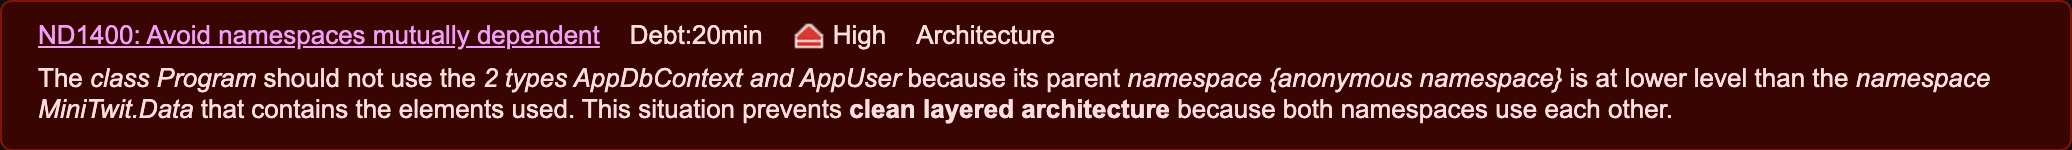
\includegraphics[width=\textwidth]{images/high-priority-rule-violation.png}
    \caption{Example - high priority rule violation}
    \label{fig:minitwit-diagram}
\end{figure}

Integrating static analysis and test coverage into the CI/CD workflow will be an important next step to enforce quality gates and prevent regressions.

\subsection{Justifications for Technology Choices}
% MSc students should argue for the choice of technologies and decisions for at least all cases for which we asked you to do so in the tasks at the end of each session.

We decided to use C\# and ASP.NET Core. This choice was partly motivated by the fact that one of the group members is very familiar with .NET and C\#, but also because the rest of the group wanted to learn and get familiar with the technology, as it is a popular choice within the industry.

With regards to the particular choice of architecture within the application, we began exploring the use of Razor pages. However, as we have a lot of shared functionality, e.g. different timelines that all look identical, but where the difference is that it is either scoped to a user, the logged in user (my timeline) or the public timeline, we wanted a more general solution that supported this unified view of a timeline. So, we landed on the use of traditional ASP.NET Core MVC. That way we could have one view for timelines and different controller actions in the backend for the three different kinds of timelines.

We chose to use an Object Relational Mapper (ORM) from the start, specifically Entity Framework Core (EF Core). The main reason for this is because EF Core is tightly integrated into the library we chose for user management called ASP.NET Core Identity\footnote{\url{https://learn.microsoft.com/en-us/aspnet/core/security/authentication/identity?view=aspnetcore-9.0&tabs=visual-studio}}. The library offers a super class called IdentityDbContext which already implements the database model for users, which we inherit from in our own AppDbContext class. Additionally, the two classes from the identity library we use for authentication, SignInManager and UserManager, make use of this database context class. So, using SQL directly from the beginning would have been an unnecessary challenge with no benefit, even though it would have been nice to have our software evolve by making the switch to an ORM throughout the development process.

\section{Process Perspective}
\subsection{CI/CD Pipeline}
% A complete description of stages and tools included in the CI/CD chains, including deployment and release of your systems.

Our ASP.NET Core web application is built and deployed using a CI/CD pipeline that integrates GitHub Actions, Docker Hub, and DigitalOcean. When code is pushed to the main branch, the pipeline triggers a workflow that runs tests (where implemented), builds a Docker image of the MiniTwit application, and pushes it to Docker Hub. In addition, two separate workflows handle application documentation and release tasks (see Figure \ref{fig:CICD-diagram}).

\begin{figure}[h!]
    \centering
    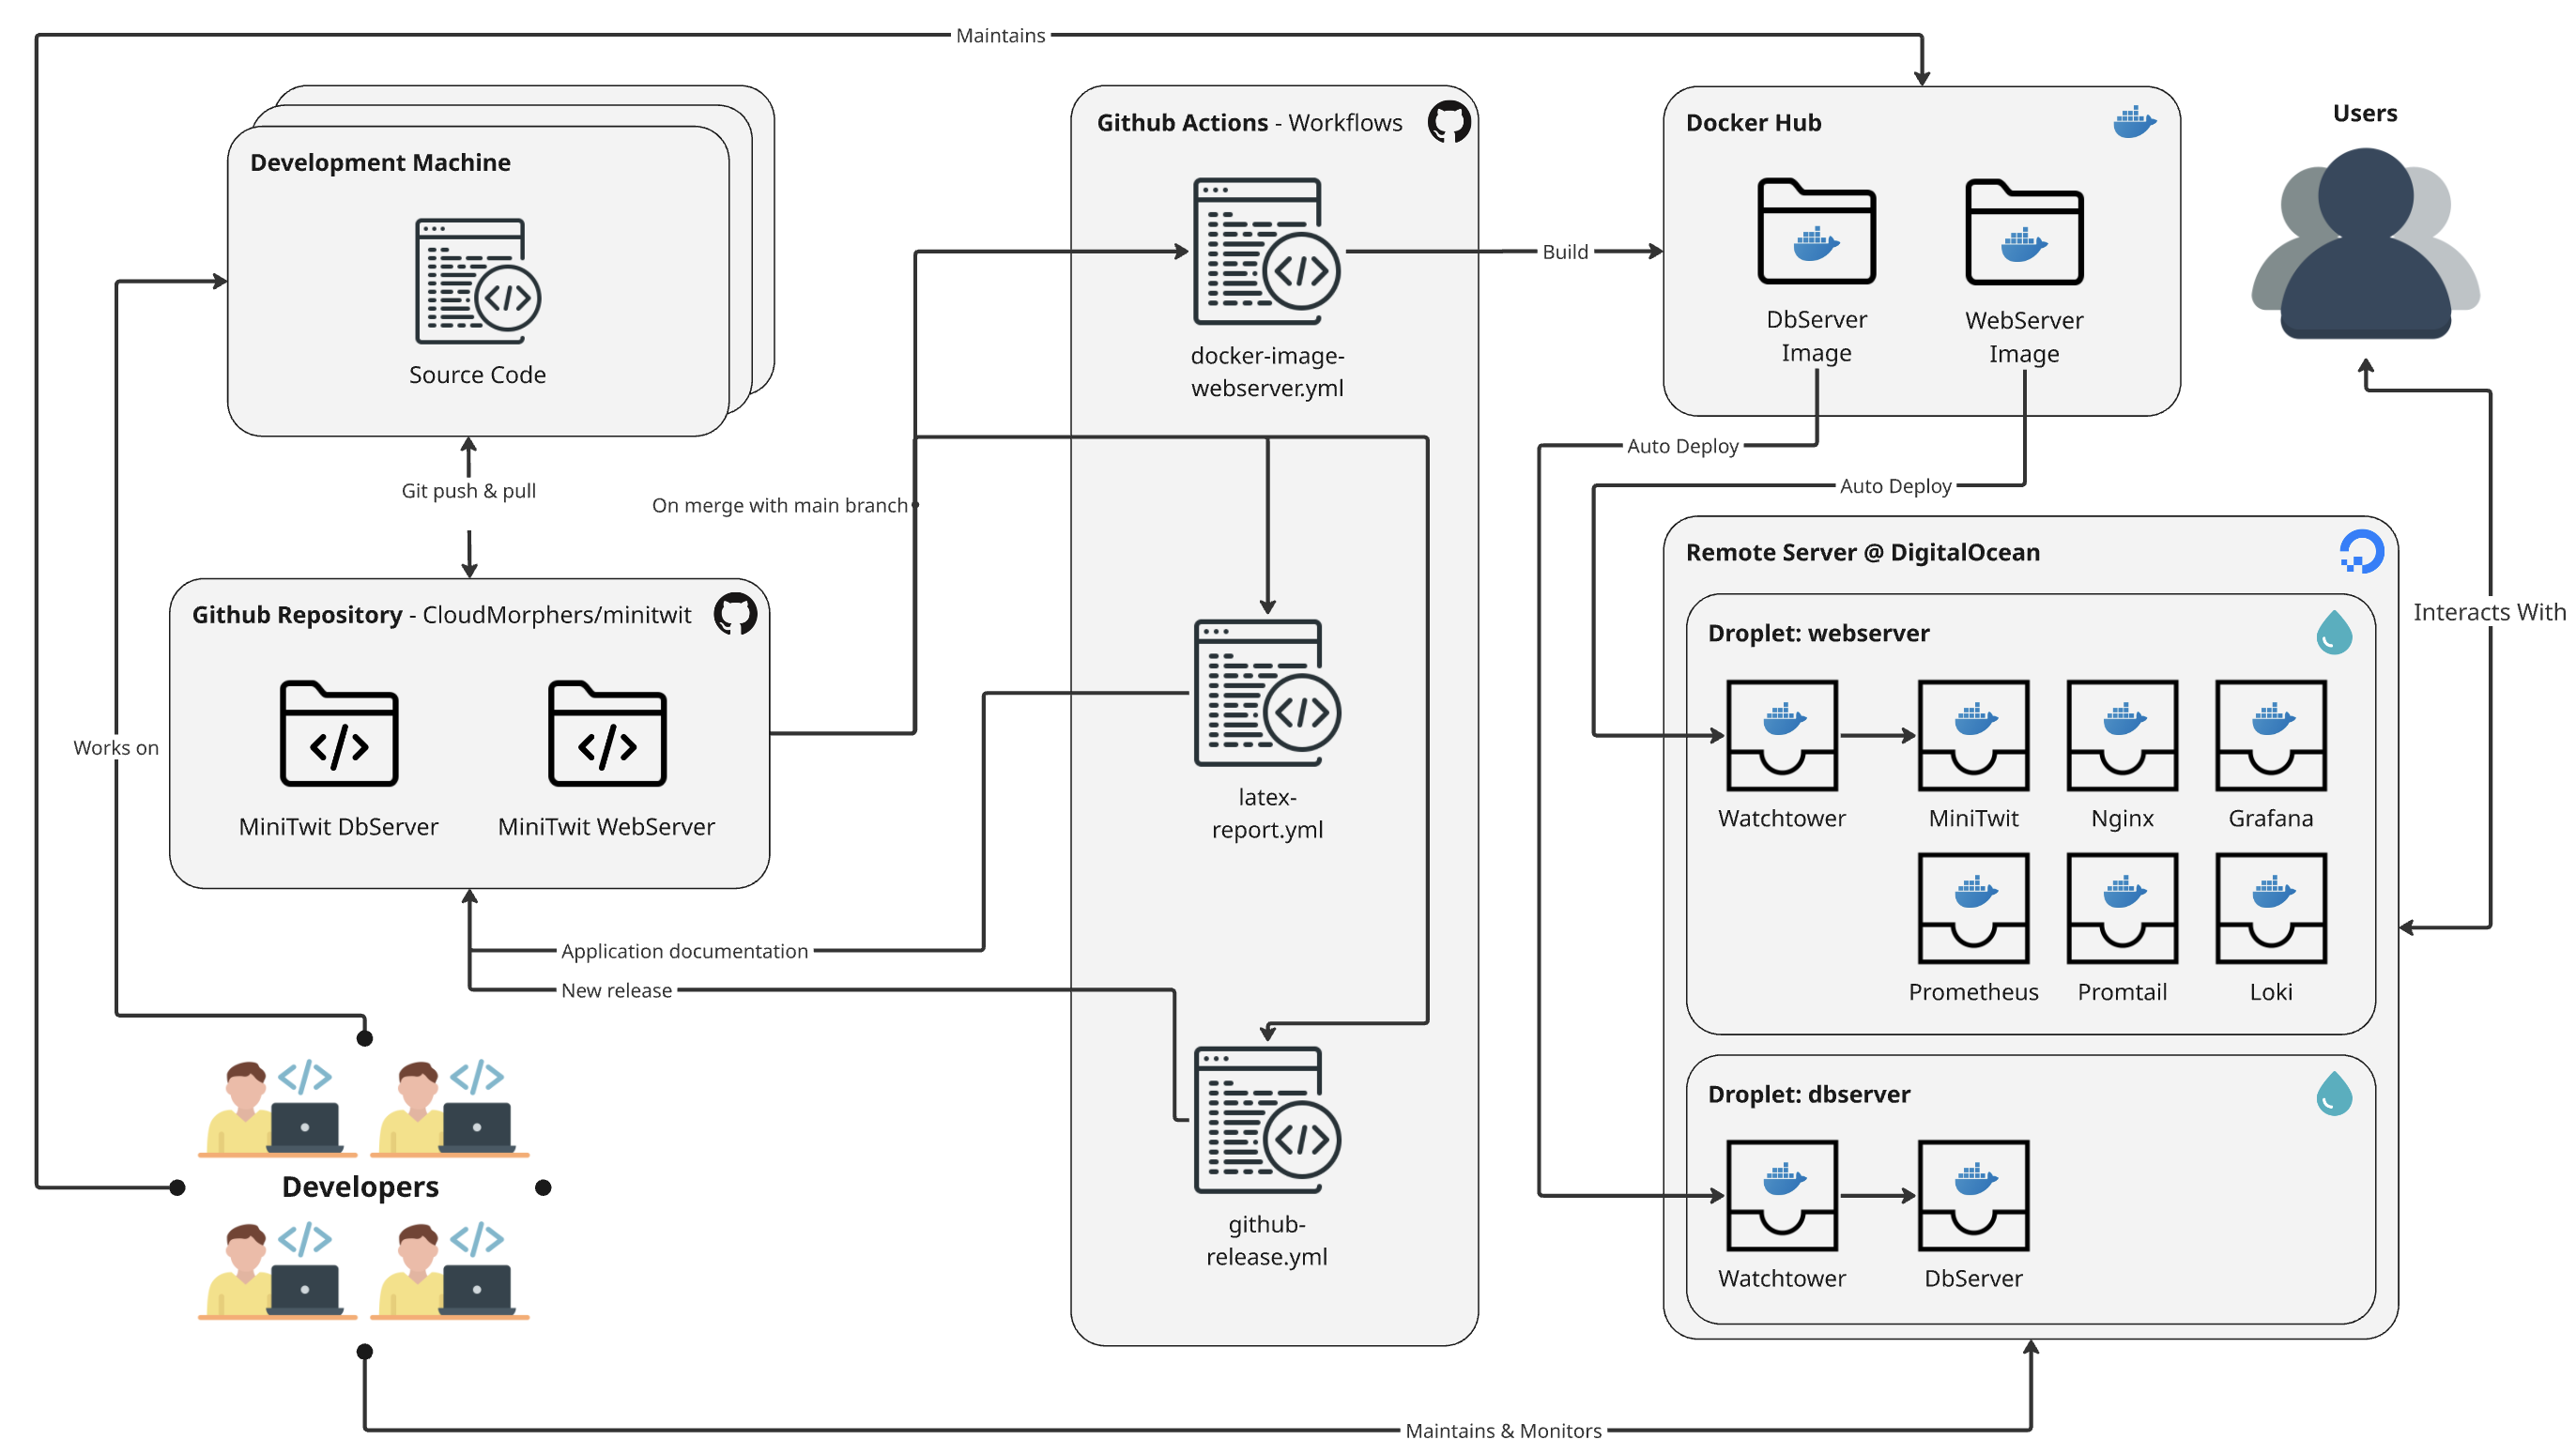
\includegraphics[width=1.0\textwidth]{images/CI_CD.png}
    \caption{CI/CD Pipeline}
    \label{fig:CICD-diagram}
\end{figure}


On our DigitalOcean server, a set of supporting Docker containers, including Watchtower, Nginx, Grafana, Prometheus, Promtail, and Loki, are launched and managed manually via docker-compose. Once running, Watchtower monitors for updated images and automatically redeployed the latest versions of the DbServer and MiniTwit containers.

While the CI/CD pipeline is largely automated, the initialization and configuration of the supporting containers still require manual SSH access to the server. Furthermore, automated testing has not yet been fully integrated into the pipeline and remains an area for future improvement.

\subsection{Monitoring}
% How do you monitor your systems and what precisely do you monitor?

We monitor our system using Prometheus and Grafana. The prometheus-net.AspNetCore package exposes application metrics at the /metrics endpoint, which Prometheus scrapes every 5 seconds to provide real-time insights into system behavior and performance.

In \href{http://67.207.72.20:3000/d/feh7hq21y4g00a/api-endpoints?orgId=1&from=now-20d&to=now&timezone=browser}{Grafana} we visualize metrics like the rate of incoming HTTP requests, helping us track the volume of API calls and their return code, in order to detect anomalies such as traffic spikes or increases in 404 errors for timely issue identification. The Grafana dashboard can be accessed \href{http://67.207.72.20:3000/d/feh7hq21y4g00a/api-endpoints?orgId=1&from=now-20d&to=now&timezone=browser}{here} with password: \texttt{Q9meuDXeCMi5G2QosWiR} and username: \texttt{admin}.

Grafana’s configuration, dashboards, and output data are stored in a dedicated grafana\_data Docker volume, ensuring they persist across container restarts without requiring reconfiguration.

\subsection{Logging}
% What do you log in your systems and how do you aggregate logs?

In our system, we log key HTTP request and response details, including request paths, status codes, and execution times. Additionally, we inject custom logs inside specific controller methods (e.g., in ApiController) to capture important actions like follow/unfollow operations, along with relevant parameters.

We use Serilog to handle logging, writing logs both to the console and to local log files under /var/log/minitwit/api/ with daily rolling. To aggregate and centralize these logs, we use Promtail to collect logs from the file system and forward them to Loki, which stores them and makes them queryable in Grafana. This setup allows us to visualize and filter logs directly within Grafana dashboards, making it easy to monitor HTTP activity, detect errors, and trace specific application events across the system.

\subsection{Security}
% Brief results of the security assessment and brief description of how did you harden the security of your system based on the analysis.

In terms of security, we have set up a firewall that blocks any incoming traffic on ports other than SSH (22) and ports that our Docker containers are set up to expose on the public IP address. We have a droplet for the website and a droplet for the PostgreSQL database. The database only needs to be accessed by the website’s backend, and thus it is unnecessary to expose it to the internet. Therefore, we opted to only have the database exposed on the internal network between our droplets, also called the Virtual Private Cloud (VPC) network. This was simply done by adding the following to the ports section in the \texttt{docker-compose} file for the database: \texttt{\$\{PRIVATE\_IP\}:5432:5432}. This ensures that the container will only use the private IP in the VPC network of the droplet, which is set in an environment variable inside an \texttt{.env} file.

Another form of security hardening we have done is to use Nginx as a reverse proxy to the website. Although the Kestrel web server of ASP.NET Core is capable of being directly exposed to the internet, it is generally considered good practice to have a reverse proxy in front. This is because Nginx is very widely used and thus can be considered more secure to have as the public-facing application (because one can assume it is more field-tested). Furthermore, it conceals the fact that we are using ASP.NET Core, as the responses being sent out to users contain Nginx headers instead.

As a final note, we did not have time to set up Transport Layer Security (TLS) or HTTPS, so all traffic going to and from clients and the web server is unencrypted. This is an issue, because if there is an adversary listening to the traffic in-between the client and the server, they will be able to record the data contained within the HTTP requests/responses, or even replace the contents to perform a Man In The Middle (MITM) attack. Sensitive data such as usernames and passwords can then be stolen and the contents of messages to be posted can be altered.

To secure our website we should have set up TLS by getting a domain name and requesting a free certificate from Let’s Encrypt. This can simply be done inside our Nginx reverse proxy, by setting it up to listen on port 443 and use the certificate from Let’s Encrypt\footnote{\url{https://letsencrypt.org/}}. Alternatively, if we were to remove Nginx, the ASP.NET Core application can also be configured to use HTTPS.

\subsection{Scaling and Upgrades}
% Applied strategy for scaling and upgrades.

While we did not manage to implement full horizontal scaling in our deployment, we planned an architecture using Docker Swarm. Our design involved deploying NGINX as a Swarm service to act as a reverse proxy and load balancer, coordinating traffic across multiple instances of our application. The intended setup included 3 manager nodes responsible for orchestrating the cluster, each connected to 2 worker nodes where the application containers would run. This approach would allow us to scale services horizontally by increasing the number of replicas on worker nodes without downtime.

\subsection{Use of AI Assistants}
% In case you have used AI-assistants during your project briefly explain which system(s) you used during the project and reflect how it supported or hindered your process.

Throughout the development of our MiniTwit system, we made use of OpenAI’s ChatGPT and GitHub Copilot to support our learning and implementation. These AI tools were particularly helpful for explaining unfamiliar concepts, such as ASP.NET Core architecture, Entity Framework behavior, and Docker configurations. We found that LLMs were most effective when used on isolated sections of code, while they struggled with broader context. This was especially true when dealing with interactions across multiple components, such as Docker container networking. Additionally, the AI sometimes generated outdated or deprecated code examples, which required us to cross-check with official documentation.

\section{Reflections}
% Describe the biggest issues, how you solved them, and which are major lessons learned with regards to:
% - evolution and refactoring
% - operation, and
% - maintenance 
% of your ITU-MiniTwit systems. Link back to respective commit messages, issues, tickets, etc. to illustrate these.

% Also reflect and describe what was the "DevOps" style of your work. For example, what did you do differently to previous development projects and how did it work?

Biggest issues
\begin{itemize}
    \item Unfamiliarity with ASP.Net Core
    \item Database migration ?
    \item ci/cd pipeline integration / from local development to containerised 
    \item Our promtail went down because there has been an overload of data that would slow down the server: The solutionL limit the amount of data that could be read in the pipeline.
\end{itemize}


\subsection{Database migration}

\subsection{Local Development - Docker Containers}
During the implementation of Docker containers for our MiniTwit application, we gradually transitioned to using containers for local testing to ensure compatibility with monitoring tools like Prometheus and Grafana. However, we encountered frequent issues, as the main application could not start without a connected database. Much of the development happened in parallel, and one group member resolved the issue by setting up a local database and configuring the necessary environment variables. Unfortunately, this solution was initially treated as a local fix and was not immediately shared with the rest of the team, resulting in lost development time. This experience taught us the importance of clear communication and proactively sharing problems and solutions within the team.

\subsection{Promtail read overload}
Toward the end of the simulation, we noticed that part of our monitoring setup had stopped working, specifically, the Loki container was no longer running. We restarted the containers, and initially, everything appeared to function as expected. Unfortunately, shortly after, the MiniTwit application crashed, and we lost the ability to SSH into the remote server and had to restart the droplet.

Given that Loki had previously failed, we restarted all containers except Loki. Surprisingly, the server quickly became so unresponsive that we could barely type commands in the SSH terminal. We then restarted the Droplet once more and brought up the containers one by one. This helped us isolate the issue to the Promtail container.

The system slowdown resembled a resource exhaustion issue. After some research, we discovered similar cases where Promtail caused performance degradation due to the absence of a read limit on log ingestion. This matched our situation, as the system had accumulated a large volume of logs over time, and Promtail was attempting to process them all at once, overloading the server in the process. This taught us the importance of setting resource limits policies to prevent monitoring tools like Promtail from overloading the system.



% \section{Bibliography}
\printbibliography[heading=none]
\end{document}